

Popsat termín BigData není úplně snadné a to z několika důvodů. Předně protože neexistuje žádná přesná definice tohoto pojmu. Tento termín je stejně jako obor, kterého se týká velice dynamický a rychle se mění. V neposlední řadě také proto, že se používá především v marketingové komunikaci jako \uv{Buzzword} za účelem vzbudit zájem čtenáře/posluchače přestože je použit v nesprávném kontextu.

Termín BigData označuje manipulaci s datasety tak velkými, že je nemožné nebo velice obtížné  s nimi manipulovat za pomocí tradičních databází ( převážně relačních) a nástrojů. Pod pojmem manipulace s datasety myslíme:

\begin{itemize}
  \item Sběr
  \item Organizce
  \item Ukládání
 \item Prohledávání
 \item Sdílení
 \item Analýza
 \item Vizualizace
\end{itemize}

Nalezení této hranice, či ji dokonce definovat je komplikovanější problém mimo rozsah této práce a na toto téma bylo napsáno mnoho jiných prací. Jak jsem zmínil v úvodu, práce se nezabývá porovnáním BigData a klasických relačních databází. 

V této kapitole se pokusím obecně přiblížit co to tedy BigData jsou, jak se liší a důvod vzniku tohoto odvětví.


\section{Trend velkých datasetů}
Ja jsem již naznačil, BigData jsou o zpracování velkých DataSetů tento trend upřednostňování velkých datasetů oproti několika menším, které v součtu mají stejný objem a informace začal vzhledem k jednodušímu hledání a objevení i zdánlivě neexistujících korelací, projevení obchodních trendů, či určování určitých jevů v reálném nebo skoro reálném čase. 

\section{3V}
Jak předchozí odstavec naznačil, BigData nejsou pouze o objemu dat jak by se mohlo zdát. Jedná se o komplexnější kategorizaci, kde hrají roli i ostatní charakteristiky, které se v literatuře značí zkratkou 3V odvozenou od počátečních písmen těchto kategorií v anglickém jazyce. 

\begin{figure}[h]
\centering
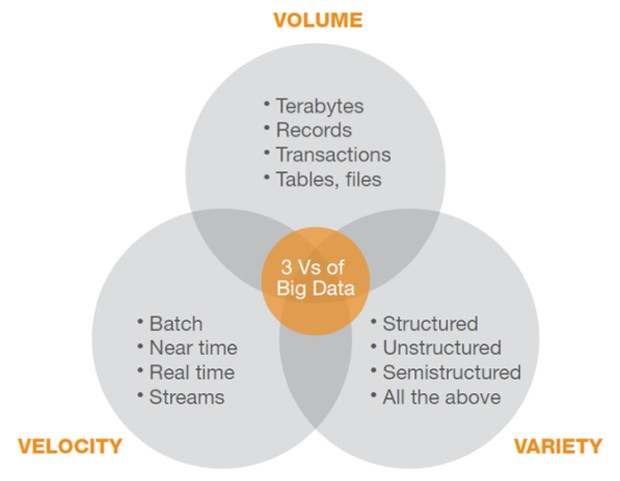
\includegraphics[scale=0.6]{images/3v}
\caption{http://smartdatacollective.com/yellowfin/75616/why-big-data-and-business-intelligence-one-direction}
\label{fig:3v}

\end{figure}

\subsection[3v-volume]{Obsah (Volume)}
Data dnes nejsou pouze v textové podobě, můžeme je uchovávat formou hudby, obrázku či videa. Vzhledem k tomuto faktu čelíme obrovskému exponenciálnímu nárůstu dat a není vyjimečné aby enterprise systémy uchovávaly Terabyty nebo Petabyty dat. Data tedy tvoří množství informaci, které jsou dost často vyhodnocovány z různých úhlů a následně uloženy a znovu vyhodnocovány a přestože původní data zůstala nezměněna, díky reevaluaci nám data rostou ohromným způsobem a takto může být na objem nahlíženo jako na jednu z charakteristik.

\subsection{Rychlost (Velocity)}
Na rychlost můžeme nahlížet hned ze dvou pohledů. Prvním jak rychle nám data přibývají a jak aktuální pro nás jsou. Například historie vývoje měnového kurzu je informace, jejíž včerejší hodnota je naprosto nevypovýdající a mění se i každou minutu. Změnila se i rychlost jakou noviny a televizní stanice získávají informace skrze sociální sítě. Data tedy rostou rychle a aktuálnost informací se rapidně zkrátila. Druhý pohled na tuto charakteristiku značí jak rychle data potřebujeme zpracovávat. Jsou informace které k nám proudí velice často například každou minutu ale jejich vyhodnocení dává smysl jednou za 24 hodin. Ale jsou také data které potřebujeme zpracovávat v reálném čase rovnou jak knám proudí. Například data z meteorologické stanice. 
Rychlost s jakou jsou data dnes potřeba zpracovat se mnohonásobně zmenšila a tedy nejen objem dat ale i rychlost zpracování reprezentuje BigData.

\subsection{Různorodost (Variety)}
Jak je z Obrázku ~\ref{fig:3v} patrné různorodost dat znamená jejich strukturovanost/nestrukturovanost. Jak bylo zmíněno, data mohou mít mnoho podob. Ale i data ve stejné podobě například textové, mohou být jinak strukturovány a tomuto faktu je potřeba se přizpůsobit a uchovávat a zpracovávat data v jiných formátech. Tato různorodost a adaptabilita je tedy poslední charakteristikou BigData

\section{BigData zjednodušeně}
Předcházející řády by měli sloužit jako shrnutí a lehký úvod do problematiky BigData. Dalo by se také říci, že BigData není jen o velkém množství dat ale je to celý koncept uchovávání a možnosti nových náhledů stávající data a také návod jak zachytit a zpracovat budoucí data. Další odstavce budou věnovány historii tohoto konceptu, ale také nejtypičtějších odvětví, kde se vyskytuje. 

\section{Historie}

Již od počátků počítačové éry byla data potřeba analyzovat. \cite{history} Avšak s rychle rostoucí dostupností technologií a jejich obecnému přijetí ve společnosti se posouvala hranice této potřeby od vladních organizací až po současnost, kdy obrovské množství informací a jejích analýzu potřebují i malé podníky

\subsection{30. a 40. léta}
V této době se použivali první počítačové simulace především ve válečném odvětví kdy například vědci z Manhattan projektu pomocí počítačových simulací, simulovali dopad a efekt jaderné bomby

\subsection{50. a 60. léta}
V tomto období se počítače a celkově zpracování a anlýza dat rozšířila o velké korporace a výzkumné laboratoře. Počítač ENIAC generoval první modely předpovědi počasí. Analytici vyřešili první problém nejkratší cesty a mnoho dalších viz. \cite{history}

\subsection{70. až 90. léta}
V této době se analytická činnost rozšířila o středně velké podniky a technologické startupy a objevují se dnes známe případy užití. První predikční model na pokles a růst akcií. První komerční nástroj pro modelově řízené rozhodování a hlavně Společnosti jako Ebay a Amazon startují svou činnost, bitva o perzonalizaci online nákupů právě začala! Google implementuje první vyhledávací algoritmus, který zvyšuje relevanci výsledků.

\subsection{2000 až součanost}
V tomto období se analytika a rozšířila až na oblast malých podniku a analytických expertů jednotlivců. Analytika začíná mít obrovský dopad na život. Dynamické změny cen zboží, doporučení produktů, hudby a filmů nebo řízení dopravy. analýza a procesování přirozeného jazyka z novin, emailů nebo sociálních sítí. Příchod Big Data, vzhledem k levné dostupnosti výpočetního výkonu a rychlosti zpracování dat, se stává tato možnost dostupnout téměř pro kohokoliv.

\subsection{Budoucnost}
V budoucnu se předpokládá, že analytická činnost se rozšíří do každodenního užití i pro jednotlivce a bude tak řídit jejich rozhodnutí. V běžném životě se také předpokládá, že analýza dat přinese například. Predikce v policejní sféře a boji proti zločinu, výzkum ve zdravotnictví nebo kompletně personalizovaná zákaznická interakce i pro malé podniky a řetězce.

\section{Nástup sociálních sítí}
Big Data zažila obrovský nástup také díky příchodu a masivnímu rozšíření sociálních sítí a to hned ze dvou důvodů. Prvním důvodem je, že nástup sociálních sítí přilálakal tisíce výzkumníků, kteří začali sbírat data z Facebooku a Twitteru a hledali různá spojeni mezi zprávami a účty z nich pak vyvozovali závěry ohledně těchto sociálních sítí. Další možností k čemu vytěžená data použivali bylo k vytváření tzv. sociálních grafů. Historicky sbírali antropologové a sociologové data o lidských vztazích skrze dotazníky, rozhovory, pozorování a experimenty. dolováním dat ze sociálních sítí, kde lidé sdílejí mnoho detailů ze svých životů se jim otevřel nový kanál, kde mají všechny tyto informace jednouše k dostání a stačí je pouze analyzovat.

BigData podle vědců představájí 2 druhy sociálních sítí: \uv{Artikulované sítě} a \uv{Behaviorální sítě}. První kategorie znázorňuje sítě, kde uživatelé zadávají své přátelé a konexe skrze technické mechanismy jako například: telefonní seznamy, emaily, seznamy přítel z jiných sití atd. Druhou kategorií jsou sítě odvozené od komunikačních vzorců. Do této skupiny spadají uživatelé, kteří si píšou zprávy nebo jsou označení na společných fotkák. Obě ty to skupiny mají pro výzkumníky velký význam přestože jím nepřikládají takovou váhu jako reálným osobním vztahům. \cite{social}

Druhým důležitýn aspektem, proč jsou sociální sítě pro Big Data důležité, je fakt, že tyto sítě samy potřebují někde svá data uchovávat a zpracovávat a proto tedy technologické týmy těchto služeb vytvářejí velké \% kolaborátorů v BigData projektech, či dokonce vytvářejí a následně uvolňují svoje technologie a nástroje k užití pro širokou veřejnost. Pro komunitu jsou důležité i přednášky a prezentované poznatky od těchto datových gigantů, kteří prozkoumavájí a prolamují lidstvu dosud známe bariéry a umožňují tím využívání technologických pokroků i jiným subjektům. 

Sociální sítě samozřejmě nejsou jediným průkopníkem na poli BigData, internetový giganti jako Google, Amazon a Yahoo také přispívají stejným dílem, na sociálních sítích je však zajímavé to, že jejich data jdou do jisté míry jednoduše dolovat a tak vzniklo mnoho spolčeností, které se začali analýzou a sběrem zabývat a způsobili tím popularizaci spojení BigData se sociálními sítěmi. 


\section{Odvětví}

Jak bylo v předchozí sekci zmíněno, v dnešní době můžeme na BigData narazit kdekoliv a v jakémkoliv odvětví. Zde bych chtěl poukázat na široké spektrum využití napříč různými činostmi, kterým se lidstvo zaobírá.\cite{sektory}

\subsection{Maloobchod}
Péče o zákazníka a samozřejmě i zvýšení zisku jsou hlavními motivy pro zpracovávání a analýzu dat. Ná základě chování uživatelů (aktivita na webu, zákaznická karta, anonymni zákazníci) předpovídat chování zákazníka v každém stádiu nákupu. Lze spojit i s podnikovými daty a hledat korelace pomocí Map Reduce mechanizmů. Největším průkopníkem spojení BigData a maloobchodu je bezesporu řetězec Tesco se svou věrnostní kartou ClubCard. Kde na základě uživatelovi nákupní historie, sestavují žebříček produktů k doporučení, či dokonce odhadují dané obdboí těhotenství svých zákaznic.\cite{tesco}

\subsection{Věda a výzkum}

Není žádným překvapením, že ve vědě a výzkumu se využívají Big Data na uchovávání výsledků z měření, či hledání korelací v naměřených výsledcích. Například držitel Nobelovy ceny Peter Higgs používal NoSQL databázový systém Cassandra na zpracování svých dat, díky nímž prokázal existenci tzv. Higgsova Bosonu \cite{higgs}

\subsection{Meteorologie}
Díky sběru a vyhodnocování dat z meteorologických stanic se podařilo vytvořit mnohem spolehlivější a přesnější modely pro předpovědi počasí a to jak dlouhodobých, tak krátkodobých. 

\subsection{Finance}
Zde je způsobů užití hned několik, například již výše zmíněné doporučování produktů, dle historie transakcí a sběru  osobních dat, banky a jiné finanční instituce navrhují vhodné finanční produkty jako například hypotéky. Druhým mnohem zajímavějším případem využití je detekce podvodů, kde jsou banky na základě analýzy všech transakcí hledat vzory podvodných chování a vyhodnotit určité transakce jako podezřelé a tím tak chránit své klienty nebo sami sebe.

\subsection{Webová optimalizace}
Na základě ukládání a následného zpracování veškěrého chování uživatele na stránce, mohou firmy optimalizovat webové stránky a jejich obsah, či ho případně restrukturalizovat. Po vyhodnocení chování konkrétních uživatelů jde obsah stránky automaticky personalisovat a podsouvat uživatelům pro ně zajímavé věci, aniž by se k nim museli proklikávat.

\subsection{BioInformatika}
V Bioinformatice se BigData využívají například k mapování genomů nebo sekvenční analýze. Tyto informace pomáhají k lepšímu pochopení DNA a také prevence genetických poruch a vrozených nemocí, či usnadnění jejich léčby. \cite{industries} 

\section{Dnešní možnosti}
V dnešní době existují v podstatě 3 možnosti jak začít s BigData. 

\subsection{Specilizované firmy a hotová řešení}
Na internetu nalezneme několik firem zabývajících se analýzou vašich dat, kde veškerá analýza a vizualizace probíhá v softwaru třetí strany. Mezi nejznámější patří společnost Good Data ycite{gooddata}. Tyto firmy se však specializují na zpracování firemních dat a vizualizaci v jejich vlastních BI nástrojích.

\subsection{Hotová enterprise řešení}
Další možností je vybrat něaké komplexní řešení od firem zabývajících se platformou BigData, která vám dodá software pro ukládání, analýzu a vizualizaci vašich dat. Programování komponent, či konfigurace je v režii zákazníka a tyto firmy poskytují licence, školení a technickou podporu. Tuto možnost postkytuje například IBM.

\subsection{Open Source a řešení z něj vycházející} 
Poslední možností je použití Open Source nástrojů, které umožní ukládat, analyzovat a vizualizovat data. Toto je cesta, kterou jsem vybral v této práci a budu se mu až do konce této práce věnovat. Drobnou nadstabou těchto řešení jsou firmy poskytující komerční balíčky těchto opensource řešení. Jedná se o velice populární přístup, pokud je potřeba zkombinovat několik nástrojů dohromady je jejich konfigurace velice obtížná a tyto komerční balíčky jsou již nakonfigurovaná hotová řešení většinou i s drobnou nadstavbou která umožnujě některé procesy a činnosti. 
